\section{Additional Related Work}


This section provides a comprehensive overview of related work beyond the concise discussion in Section 2.

\subsection{Evolution of RAG Systems}

The development of retrieval-augmented generation has seen significant advances beyond the foundational work. REALM \cite{guu2020retrieval} pioneered retrieval-enhanced pre-training, while dense retrieval methods \cite{karpukhin2020dense} and efficient architectures like ColBERT \cite{khattab2020colbert} improved retrieval quality. 

Recent innovations have introduced more sophisticated strategies. RICHES \cite{jain2024ragriches} unifies retrieval with generation by directly decoding document contents, eliminating the need for separate retriever and generator components. Multi-Level Information RAG \cite{adjali2024multilevel} enhances answer generation through entity retrieval and query expansion with joint-training loss. These advances demonstrate the field's progression toward more integrated and efficient architectures, though none address version-specific challenges.

\subsection{Graph-Based Retrieval Systems}

Beyond GraphRAG, several systems have explored graph-enhanced retrieval. TRACE \cite{fang2024trace} employs a KG Generator to create knowledge graphs from retrieved documents and constructs reasoning chains for multi-hop QA, achieving up to 14.03\% improvement over baseline methods. Knowledge Graph-Enhanced LLMs \cite{li2024kgframework} use question decomposition and atomic retrieval to improve reasoning over structured knowledge. Q-KGR \cite{zhang2024qkgr} introduces question-guided re-scoring to eliminate noisy pathways in retrieved subgraphs.

While these approaches demonstrate the value of graph-based reasoning, they focus on semantic relationships rather than temporal or version-specific connections. The computational costs remain significant—our analysis shows GraphRAG requires 11,761 nodes and 39,438 relationships for our test corpus, while VersionRAG achieves superior accuracy with only 896 nodes.

\subsection{Temporal Reasoning in NLP}

Temporal reasoning has been extensively studied across different aspects. TimeR$^4$ \cite{qian2024timer4} integrates temporal knowledge from Temporal Knowledge Graphs into LLMs through a Time-aware Retrieve-Rewrite-Retrieve-Rerank framework, achieving 47.8\% and 22.5\% relative gains on temporal reasoning tasks. Time Matters \cite{barik2024timematters} addresses temporal claim verification by extracting temporal cues and applying temporal reasoning for fact-checking. Natural Evolution-based approaches \cite{chen2024natural} model asynchronous characteristics of event evolution in temporal KGs using dual-level aggregation.

These approaches focus on continuous temporal dimensions (dates, time periods) rather than discrete version numbers. The distinction is crucial: version transitions in technical documentation follow semantic versioning conventions (major.minor.patch) that encode compatibility and change severity, which temporal reasoning systems cannot capture.

\subsection{Domain Adaptation in RAG}

Several recent works have explored adapting RAG to specific domains. RAG-Studio \cite{mao2024ragstudio} generates domain-specific training data through self-alignment, fine-tuning both LLMs and retrievers to work cohesively for domain-specific tasks. LongRAG \cite{zhao2024longrag} introduces a dual-perspective paradigm for long-context QA, processing information at both global and local levels to handle documents up to 100K tokens. Unified Active Retrieval \cite{cheng2024unified} addresses the challenge of when to retrieve through multiple orthogonal criteria, achieving better retrieval timing judgments with negligible extra inference cost.

While these systems improve domain-specific performance, they do not address the fundamental challenge of document versioning where the same query may have different answers depending on the version context.

\subsection{RAG Evaluation and Analysis}

The evaluation of RAG systems has become increasingly sophisticated. ARES \cite{saadf2024ares} provides an automated evaluation framework using synthetic training data and lightweight LM judges to assess context relevance, answer faithfulness, and answer relevance. A comprehensive study \cite{li2024raglongcontext} comparing RAG with long-context LLMs reveals that while long-context models achieve better average performance when sufficiently resourced, RAG maintains a significant cost advantage—particularly relevant given VersionRAG's 97\% reduction in indexing tokens.

Privacy and security concerns have also emerged. Research on privacy issues in RAG \cite{zeng2024privacy} demonstrates vulnerabilities in leaking private retrieval databases, highlighting the need for careful system design—an aspect we address through VersionRAG's structured graph approach that maintains clear data provenance.

\subsection{Historical Context: Early Temporal Work}

While not directly comparable to modern neural approaches, early work in temporal information retrieval laid important foundations. Research on temporal question answering in the pre-neural era established taxonomies of temporal questions and identified key challenges in handling time-sensitive information. These insights inform our query classification system, though the technical approaches differ substantially given advances in neural architectures and the specific challenge of versioned documents.


\section{Extended Experimental Results}

\subsection{Detailed Performance Breakdown}

Table~\ref{tab:detailed_breakdown} presents the complete accuracy breakdown across all query subcategories from the thesis evaluation.

\begin{table}[hb]
\centering
\small
\caption{Detailed accuracy breakdown. CR: Content Retrieval, CR-C: Content Retrieval Complex, CR-VS: Content Retrieval Version-Specific, VLI: Version Listing \& Inquiry, Ch-E: Change Explicit, Ch-I: Change Implicit.}
\begin{tabular}{llcccccc}
\hline
LLM & Approach & CR & CR-C & CR-VS & VLI & Ch-E & Ch-I \\
& & [\%] & [\%] & [\%] & [\%] & [\%] & [\%] \\ \hline
\multirow{3}{*}{DeepSeek-R1 70B} 
& Baseline & 95.0 & 80.0 & 55.0 & 35.0 & 50.0 & 0.0 \\
& GraphRAG & 85.0 & 80.0 & 100.0 & 80.0 & 50.0 & 10.0 \\
& VersionRAG & 100.0 & 80.0 & 100.0 & 100.0 & 80.0 & 60.0 \\ \hline
\multirow{3}{*}{GPT-4o Mini} 
& Baseline & 85.0 & 75.0 & 50.0 & 20.0 & 60.0 & 10.0 \\
& GraphRAG & 70.0 & 65.0 & 50.0 & 65.0 & 60.0 & 10.0 \\
& VersionRAG & 80.0 & 90.0 & 70.0 & 90.0 & 90.0 & 40.0 \\ \hline
\multirow{3}{*}{Llama 3 8B} 
& Baseline & 65.0 & 80.0 & 40.0 & 25.0 & 50.0 & 0.0 \\
& GraphRAG & 70.0 & 25.0 & 40.0 & 70.0 & 20.0 & 0.0 \\
& VersionRAG & 65.0 & 80.0 & 40.0 & 70.0 & 30.0 & 10.0 \\ \hline
\end{tabular}
\label{tab:detailed_breakdown}
\end{table}

\subsection{Query Classification Performance}

The accuracy of query intent classification directly impacts VersionRAG's routing mechanism:

\begin{table}[hb]
\centering
\small
\caption{Query classification accuracy showing smaller models struggle with change retrieval identification.}
\begin{tabular}{lcccc}
\hline
LLM & Overall [\%] & Content Retrieval [\%] & Version Listing [\%] & Change Retrieval [\%] \\ \hline
DeepSeek-R1 70B & 92.0 & 93.3 & 90.0 & 90.0 \\
GPT-4o Mini & 91.0 & 95.0 & 85.0 & 85.0 \\
Llama 3 8B & 76.0 & 73.3 & 95.0 & 65.0 \\ \hline
\end{tabular}
\end{table}

\newpage

\subsection{Resource Consumption Comparison}

Table~\ref{tab:resource_comparison} shows the dramatic efficiency difference between approaches:

\begin{table}[ht]
\centering
\small
\caption{Resource consumption showing VersionRAG's 97\% reduction in tokens and 92\% reduction in processing time.}
\begin{tabular}{llrrrr}
\hline
LLM & Approach & Input [K] & Output [K] & Cost [\$] & Time \\ \hline
\multirow{2}{*}{DeepSeek-R1 70B} 
& GraphRAG & 2,970 & 5,922 & 6.67 & 5h 12min \\
& VersionRAG & 186 & 38 & 0.17 & 25min \\ \hline
\multirow{2}{*}{GPT-4o Mini} 
& GraphRAG & 2,970 & 1,631 & 1.42 & 2h 45min \\
& VersionRAG & 184 & 54 & 0.07 & 20min \\ \hline
\multirow{2}{*}{Llama 3 8B} 
& GraphRAG & 2,970 & 2,541 & 0.35 & 2h 11min \\
& VersionRAG & 194 & 32 & 0.01 & 24min \\ \hline
\end{tabular}
\label{tab:resource_comparison}
\end{table}

\subsection{Graph Structure Statistics}

Comparison of graph structures generated by different approaches shown in Table \ref{tab:graph_structure_stats}.

\begin{table}[hb]
\centering
\small
\caption{Graph statistics showing VersionRAG's compact structure (896 nodes) versus GraphRAG's expansive graph (11,761+ nodes).}
\begin{tabular}{lrrrr}
\hline
\textbf{VersionRAG} & Total Nodes & Differ Nodes & Extract Nodes & Relationships \\ \hline
DeepSeek-R1 70B & 896 & 146 & 642 & 922 \\
GPT-4o Mini & 893 & 142 & 643 & 919 \\
Llama 3 8B & 776 & 85 & 584 & 801 \\ \hline
\textbf{GraphRAG} & Total Nodes & \multicolumn{2}{c}{Relationships} \\ \hline
DeepSeek-R1 70B & 11,761 & \multicolumn{2}{c}{39,438} \\
GPT-4o Mini & 13,236 & \multicolumn{2}{c}{31,894} \\
Llama 3 8B & 11,231 & \multicolumn{2}{c}{24,538} \\ \hline
\end{tabular}
\label{tab:graph_structure_stats}
\end{table}

\subsection{Cross-Model Indexing and Retrieval}

Complete results when using different LLMs for indexing versus retrieval listed in Table \ref{tab:cross_model_performance}.

\begin{table}[hb]
\centering
\small
\caption{Cross-model performance showing self-combinations achieve highest accuracy.}
\begin{tabular}{llcccc}
\hline
Indexing LLM & Retrieval LLM & Overall [\%] & Content [\%] & Version [\%] & Change [\%] \\ \hline
Llama 3 8B & Llama 3 8B & 55.0 & 61.6 & 70.0 & 20.0 \\
Llama 3 8B & GPT-4o Mini & 67.0 & 65.0 & 75.0 & 65.0 \\
Llama 3 8B & DeepSeek-R1 70B & 74.0 & 76.6 & 85.0 & 55.0 \\ \hline
GPT-4o Mini & Llama 3 8B & 54.0 & 51.6 & 90.0 & 25.0 \\
GPT-4o Mini & GPT-4o Mini & 79.0 & 80.0 & 90.0 & 65.0 \\
GPT-4o Mini & DeepSeek-R1 70B & 79.0 & 83.3 & 90.0 & 55.0 \\ \hline
DeepSeek-R1 70B & Llama 3 8B & 68.0 & 75.0 & 60.0 & 55.0 \\
DeepSeek-R1 70B & GPT-4o Mini & 78.0 & 76.6 & 95.0 & 65.0 \\
DeepSeek-R1 70B & DeepSeek-R1 70B & 90.0 & 93.3 & 100.0 & 70.0 \\ \hline
\end{tabular}
\label{tab:cross_model_performance}
\end{table}

\newpage

\subsection{Change Retrieval Breakdown}

Detailed performance on explicit versus implicit change detection in Table \ref{tab:change_retrieval_breakdown}.

\begin{table}[h]
\centering
\small
\caption{Change retrieval showing implicit changes are significantly harder to detect.}
\begin{tabular}{llcc}
\hline
Indexing LLM & Retrieval LLM & Explicit [\%] & Implicit [\%] \\ \hline
Llama 3 8B & Llama 3 8B & 30.0 & 10.0 \\
Llama 3 8B & GPT-4o Mini & 90.0 & 40.0 \\
Llama 3 8B & DeepSeek-R1 70B & 70.0 & 40.0 \\ \hline
GPT-4o Mini & Llama 3 8B & 50.0 & 0.0 \\
GPT-4o Mini & GPT-4o Mini & 90.0 & 40.0 \\
GPT-4o Mini & DeepSeek-R1 70B & 100.0 & 10.0 \\ \hline
DeepSeek-R1 70B & Llama 3 8B & 80.0 & 30.0 \\
DeepSeek-R1 70B & GPT-4o Mini & 80.0 & 50.0 \\
DeepSeek-R1 70B & DeepSeek-R1 70B & 80.0 & 60.0 \\ \hline
\end{tabular}
\label{tab:change_retrieval_breakdown}
\end{table}


\subsection{GraphRAG with Alternative Indexing}

Testing whether GraphRAG's limitations stem from indexing or retrieval in Table \ref{tab:graphrag_alternative_indexing}.

\begin{table}[hb]
\centering
\small
\caption{GraphRAG performance showing marginal improvement (+4\%) with better indexing.}
\begin{tabular}{llc}
\hline
Indexing LLM & Retrieval/Generation LLM & Overall Accuracy [\%] \\ \hline
Llama 3 8B & Llama 3 8B & 43.0 \\
DeepSeek-R1 70B & Llama 3 8B & 47.0 \\ \hline
\end{tabular}
\label{tab:graphrag_alternative_indexing}
\end{table}





\subsection{Document Coverage}

The dataset covers four main documentation sources listed in Table \ref{tab:document_coverage}.

\begin{table}[hb]
\centering
\small
\caption{Document coverage in VersionQA dataset.}
\begin{tabular}{llcc}
\hline
\textbf{Topic} & \textbf{Type} & \textbf{Files} & \textbf{Pages} \\ \hline
Apache Spark Releases & Changelog & 6 & ~150 \\
Bootstrap Releases & Changelog & 6 & ~120 \\
Node.js Assert Module & Documentation & 13 & ~260 \\
Node.js Errors & Documentation & 9 & ~180 \\ \hline
\textbf{Total} & & \textbf{34} & \textbf{710} \\ \hline
\end{tabular}
\label{tab:document_coverage}
\end{table}


\newpage


\section{Additional Ablation Studies}

\subsection{Cross-Model Indexing and Retrieval Performance}

Table~\ref{tab:cross_model_full} shows the complete results when using different LLMs for indexing versus retrieval/generation, revealing how indexing quality affects downstream performance.

\begin{table}[h]
\centering
\small
\caption{Complete cross-model performance matrix showing that self-combinations generally achieve highest accuracy.}
\begin{tabular}{llccccc}
\hline
Indexing & Retrieval & Overall & Content & Version & Change \\
LLM & LLM & [\%] & Retrieval [\%] & Listing [\%] & Retrieval [\%] \\ \hline
Llama 3 8B & Llama 3 8B & 55.0 & 61.6 & 70.0 & 20.0 \\
Llama 3 8B & GPT-4o Mini & 67.0 & 65.0 & 75.0 & 65.0 \\
Llama 3 8B & DeepSeek-R1 70B & 74.0 & 76.6 & 85.0 & 55.0 \\ \hline
GPT-4o Mini & Llama 3 8B & 54.0 & 51.6 & 90.0 & 25.0 \\
GPT-4o Mini & GPT-4o Mini & 79.0 & 80.0 & 90.0 & 65.0 \\
GPT-4o Mini & DeepSeek-R1 70B & 79.0 & 83.3 & 90.0 & 55.0 \\ \hline
DeepSeek-R1 70B & Llama 3 8B & 68.0 & 75.0 & 60.0 & 55.0 \\
DeepSeek-R1 70B & GPT-4o Mini & 78.0 & 76.6 & 95.0 & 65.0 \\
DeepSeek-R1 70B & DeepSeek-R1 70B & 90.0 & 93.3 & 100.0 & 70.0 \\ \hline
\end{tabular}
\label{tab:cross_model_full}
\end{table}

\subsection{Detailed Change Retrieval Performance}

Table~\ref{tab:change_detailed} breaks down change retrieval into explicit and implicit categories across model combinations.

\begin{table}[hb]
\centering
\small
\caption{Change retrieval performance showing explicit changes are easier to retrieve than implicit ones.}
\begin{tabular}{llcc}
\hline
Indexing LLM & Retrieval LLM & Change Explicit [\%] & Change Implicit [\%] \\ \hline
Llama 3 8B & Llama 3 8B & 30.0 & 10.0 \\
Llama 3 8B & GPT-4o Mini & 90.0 & 40.0 \\
Llama 3 8B & DeepSeek-R1 70B & 70.0 & 40.0 \\ \hline
GPT-4o Mini & Llama 3 8B & 50.0 & 0.0 \\
GPT-4o Mini & GPT-4o Mini & 90.0 & 40.0 \\
GPT-4o Mini & DeepSeek-R1 70B & 100.0 & 10.0 \\ \hline
DeepSeek-R1 70B & Llama 3 8B & 80.0 & 30.0 \\
DeepSeek-R1 70B & GPT-4o Mini & 80.0 & 50.0 \\
DeepSeek-R1 70B & DeepSeek-R1 70B & 80.0 & 60.0 \\ \hline
\end{tabular}
\label{tab:change_detailed}
\end{table}

\subsection{GraphRAG Performance with Different Indexing Models}

As noted in Section 4.2.3, we tested whether GraphRAG's poor performance with Llama 3 8B stemmed from indexing or retrieval limitations.

\begin{table}[h]
\centering
\small
\caption{GraphRAG performance showing that better indexing provides only marginal improvement (+4\%) when paired with a weak retrieval model.}
\begin{tabular}{llc}
\hline
Indexing LLM & Retrieval/Generation LLM & Overall Accuracy [\%] \\ \hline
Llama 3 8B & Llama 3 8B & 43.0 \\
DeepSeek-R1 70B & Llama 3 8B & 47.0 \\ \hline
\end{tabular}
\label{tab:graphrag_different_indexing_models}
\end{table}

\newpage

\subsection{Query Classification Accuracy by Model}

The accuracy of retrieval mode derivation directly impacts VersionRAG's performance as shown in Table \ref{tab:query_classification_accuracy_by_model}.

\begin{table}[h]
\centering
\small
\caption{Query intent classification accuracy showing that smaller models struggle particularly with change retrieval queries.}
\begin{tabular}{lcccc}
\hline
LLM & Overall [\%] & Content Retrieval [\%] & Version Listing [\%] & Change Retrieval [\%] \\ \hline
DeepSeek-R1 70B & 92.0 & 93.3 & 90.0 & 90.0 \\
GPT-4o Mini & 91.0 & 95.0 & 85.0 & 85.0 \\
Llama 3 8B & 76.0 & 73.3 & 95.0 & 65.0 \\ \hline
\end{tabular}
\label{tab:query_classification_accuracy_by_model}
\end{table}

\subsection{Graph Structure Complexity by Model}

Different LLMs produce varying graph structures during indexing as shown in Table \ref{tab:graph_structure_complexity_by_model}.

\begin{table}[ht]
\centering
\small
\caption{Graph structure statistics showing VersionRAG's focused approach versus GraphRAG's comprehensive entity extraction.}
\begin{tabular}{lcccc}
\hline
\textbf{VersionRAG Graphs} & Total Nodes & Differ Nodes & Extraction Nodes & Relationships \\ \hline
DeepSeek-R1 70B & 896 & 146 & 642 & 922 \\
GPT-4o Mini & 893 & 142 & 643 & 919 \\
Llama 3 8B & 776 & 85 & 584 & 801 \\ \hline
\textbf{GraphRAG Graphs} & Total Nodes & Entity Nodes & & Relationships \\ \hline
DeepSeek-R1 70B & 11,761 & 11,761 & - & 39,438 \\
GPT-4o Mini & 13,236 & 13,236 & - & 31,894 \\
Llama 3 8B & 11,231 & 11,231 & - & 24,538 \\ \hline
\end{tabular}
\label{tab:graph_structure_complexity_by_model}
\end{table}


\section{Qualitative Analysis}

\subsection{Retrieval Process Examples}

We illustrate the qualitative differences between approaches through concrete examples from our experiments.

\subsubsection{Version-Specific Content Retrieval}

When asked "What is the stability level of the assert.partialDeepStrictEqual method in Node.js version 23.11.0?", the baseline RAG system retrieves semantically similar chunks from multiple versions:
\begin{itemize}
    \item "assert.partialDeepStrictEqual method is 1\_2 - Release candidate" (v23.11.0)
    \item "assert.partialDeepStrictEqual method is 1\_0 - Early development" (v22.14.0)
\end{itemize}

This conflicting information prevents correct answer generation. In contrast, VersionRAG:
\begin{enumerate}
    \item Classifies the query as version-specific content retrieval
    \item Extracts the version parameter (23.11.0)
    \item Constrains vector search to that specific version
    \item Returns only the correct information
\end{enumerate}

\subsubsection{Change Detection}

VersionRAG successfully identifies both explicit and implicit changes:

\textbf{Explicit (from changelog):} "Upgraded Avro to version 1.11.4" (Apache Spark 3.5.5)

\textbf{Implicit (from diff analysis):} "Added new method assert.partialDeepStrictEqual" (detected between Node.js 21.7.3 → 22.14.0)

GraphRAG fails on implicit changes (10\% accuracy) because its entity-relationship extraction cannot capture transitions not explicitly stated in text.

\subsection{Graph Structure Analysis}

VersionRAG's focused graph structure enables efficient retrieval as shown in Table \ref{tab:graph_structure_analysis}.

\begin{table}[h]
\centering
\small
\caption{Resource comparison showing VersionRAG's 13× smaller graph achieves 26 points higher accuracy.}
\begin{tabular}{lcc}
\hline
\textbf{Component} & \textbf{VersionRAG} & \textbf{GraphRAG} \\ \hline
Total Nodes & 896 & 11,761 \\
Relationships & 922 & 39,438 \\
Processing Tokens & 186K & 2,970K \\
Indexing Time & 25 min & 312 min \\ \hline
\end{tabular}
\label{tab:graph_structure_analysis}
\end{table}

\subsection{Failure Mode Analysis}

Analysis of errors reveals distinct patterns:

\paragraph{VersionRAG Failures (10\% of queries).}
\begin{itemize}
    \item Query misclassification (8\%): Ambiguous queries incorrectly routed
    \item Incomplete change extraction (2\%): Subtle modifications missed by diff analysis
\end{itemize}

\paragraph{GraphRAG Failures (36\% of queries).}
\begin{itemize}
    \item Version confusion (20\%): Cannot distinguish between temporally different states
    \item Missing change detection (16\%): No mechanism for implicit change identification
\end{itemize}

\paragraph{Baseline RAG Failures (42\% of queries).}
\begin{itemize}
    \item Version mixing (25\%): Retrieves conflicting information from multiple versions
    \item No change awareness (17\%): Cannot identify modifications between documents
\end{itemize}

\subsection{Model Capacity Effects}

Smaller models show degraded performance in specific areas:
\begin{itemize}
    \item \textbf{Change extraction}: Llama 3 8B generates 42\% fewer change nodes than DeepSeek-R1 70B
    \item \textbf{Query classification}: 24\% misclassification rate with Llama 3 8B versus 8\% with DeepSeek-R1 70B
    \item \textbf{Context integration}: Limited 8,192 token window constrains complex reasoning
\end{itemize}

\subsection{Efficiency-Performance Trade-off}

VersionRAG achieves superior accuracy while requiring 97\% fewer resources than GraphRAG. This efficiency stems from encoding version relationships as explicit graph edges rather than discovering them through expensive LLM analysis. The focused graph structure (896 nodes) provides better signal-to-noise ratio than GraphRAG's comprehensive entity graph (11,761 nodes), demonstrating that domain-specific design outperforms general-purpose approaches for specialized tasks.





\newpage

\section{Implementation Details}
\label{app:implementation_details}

\subsection{System Architecture and Tools}

VersionRAG was implemented using the following tools as specified in the experimental setup:

\begin{itemize}
    \item \textbf{Llama 3 8B}: Transformer-based model with 8 billion parameters, 8,192 token context window
    \item \textbf{DeepSeek-R1 70B}: Distilled LLaMA-based model with ~70 billion parameters, 128,000 token context window
    \item \textbf{GPT-4o Mini}: Fast and cost-efficient model (context window undisclosed)
    \item \textbf{GPT-4.1}: Used specifically for LLM-as-a-judge evaluation
    \item \textbf{text-embedding-3-small}: OpenAI embedding model for all text representations
    \item \textbf{Milvus Lite v2.4.11}: Vector database for storing embeddings
    \item \textbf{Neo4j v1.6.1}: Locally hosted graph database for VersionRAG implementation
    \item \textbf{Neo4j AuraDB}: Cloud-based graph database used for GraphRAG
\end{itemize}

\subsection{Document Processing}

\paragraph{Input Formats.}
The system supports both PDF and Markdown files as input. All PDF documents are converted to Markdown format to preserve structural information while enabling text processing.

\paragraph{Chunking Configuration.}
Documents are segmented into:
\begin{itemize}
    \item \textbf{Chunk size}: 512 tokens
    \item \textbf{Chunk overlap}: 50 tokens
    \item \textbf{Purpose}: Balances context preservation with model token limits
\end{itemize}

\subsection{Indexing Process Details}

\paragraph{Attribute Extraction.}
Each document's first page is processed by an LLM to extract:
\begin{itemize}
    \item Topic title
    \item Brief content summary
    \item Version information
\end{itemize}
At least the first ten pages are analyzed to determine whether the document is a changelog or general documentation.

\paragraph{Document Clustering.}
Documents are clustered using an LLM instructed to group based on:
\begin{itemize}
    \item Title similarity for version grouping
    \item Topic similarity for category assignment
\end{itemize}

\paragraph{Change Detection.}
Two methods are employed:
\begin{itemize}
    \item \textbf{Explicit changes}: Extracted from documents identified as changelogs using LLM analysis
    \item \textbf{Implicit changes}: Detected using the DeepDiff library for line-level comparison between consecutive versions, with LLM interpretation of the differences
\end{itemize}

\subsection{LLM Configuration}

\paragraph{Prompting Strategy.}
All LLM tasks use few-shot prompting without fine-tuning. Example input-output pairs guide the model's behavior for:
\begin{itemize}
    \item Query classification into three categories (VersionRetrieval, ChangeRetrieval, ContentRetrieval)
    \item Parameter extraction (category, document, version)
    \item Change interpretation from diff outputs
\end{itemize}

\paragraph{API Access.}
\begin{itemize}
    \item GPT-4o Mini: Accessed via OpenAI API
    \item Llama 3 8B and DeepSeek-R1 70B: Accessed via GroqCloud
\end{itemize}

\subsection{Retrieval Configuration}

\paragraph{Query Classification.}
User queries are classified into three retrieval modes with the following accuracy:
\begin{itemize}
    \item DeepSeek-R1 70B: 92\% classification accuracy
    \item GPT-4o Mini: 91\% classification accuracy
    \item Llama 3 8B: 76\% classification accuracy
\end{itemize}

\paragraph{Retrieval Strategies by Query Type.}
\begin{itemize}
    \item \textbf{VersionRetrieval}: Graph traversal to version nodes
    \item \textbf{ChangeRetrieval}: Semantic search over change nodes or direct graph access
    \item \textbf{ContentRetrieval}: Vector similarity search with optional version filtering
\end{itemize}

\newpage

\subsection{Baseline RAG Implementation}

Following standard RAG methodology:
\begin{itemize}
    \item Documents chunked into 512-token segments
    \item Embeddings generated using text-embedding-3-small
    \item Top-5 chunks retrieved based on cosine similarity
    \item No version awareness or metadata filtering
\end{itemize}

The baseline implementation serves as a minimal, naive RAG setup that enables direct comparison with more advanced approaches. Each document is split into fixed-size chunks, embedded, and stored in a vector database for semantic retrieval. At query time, the top-\textit{k} semantically similar chunks are retrieved purely based on cosine similarity, without the use of metadata or contextual filtering. 

The overall structure of this baseline pipeline is illustrated in Figure~\ref{fig:BaselineRAGFramework}. This setup establishes a consistent foundation for evaluating the benefits of graph-based retrieval.

\begin{figure}[h]
    \caption{Baseline Naive RAG Framework}
    \centering
    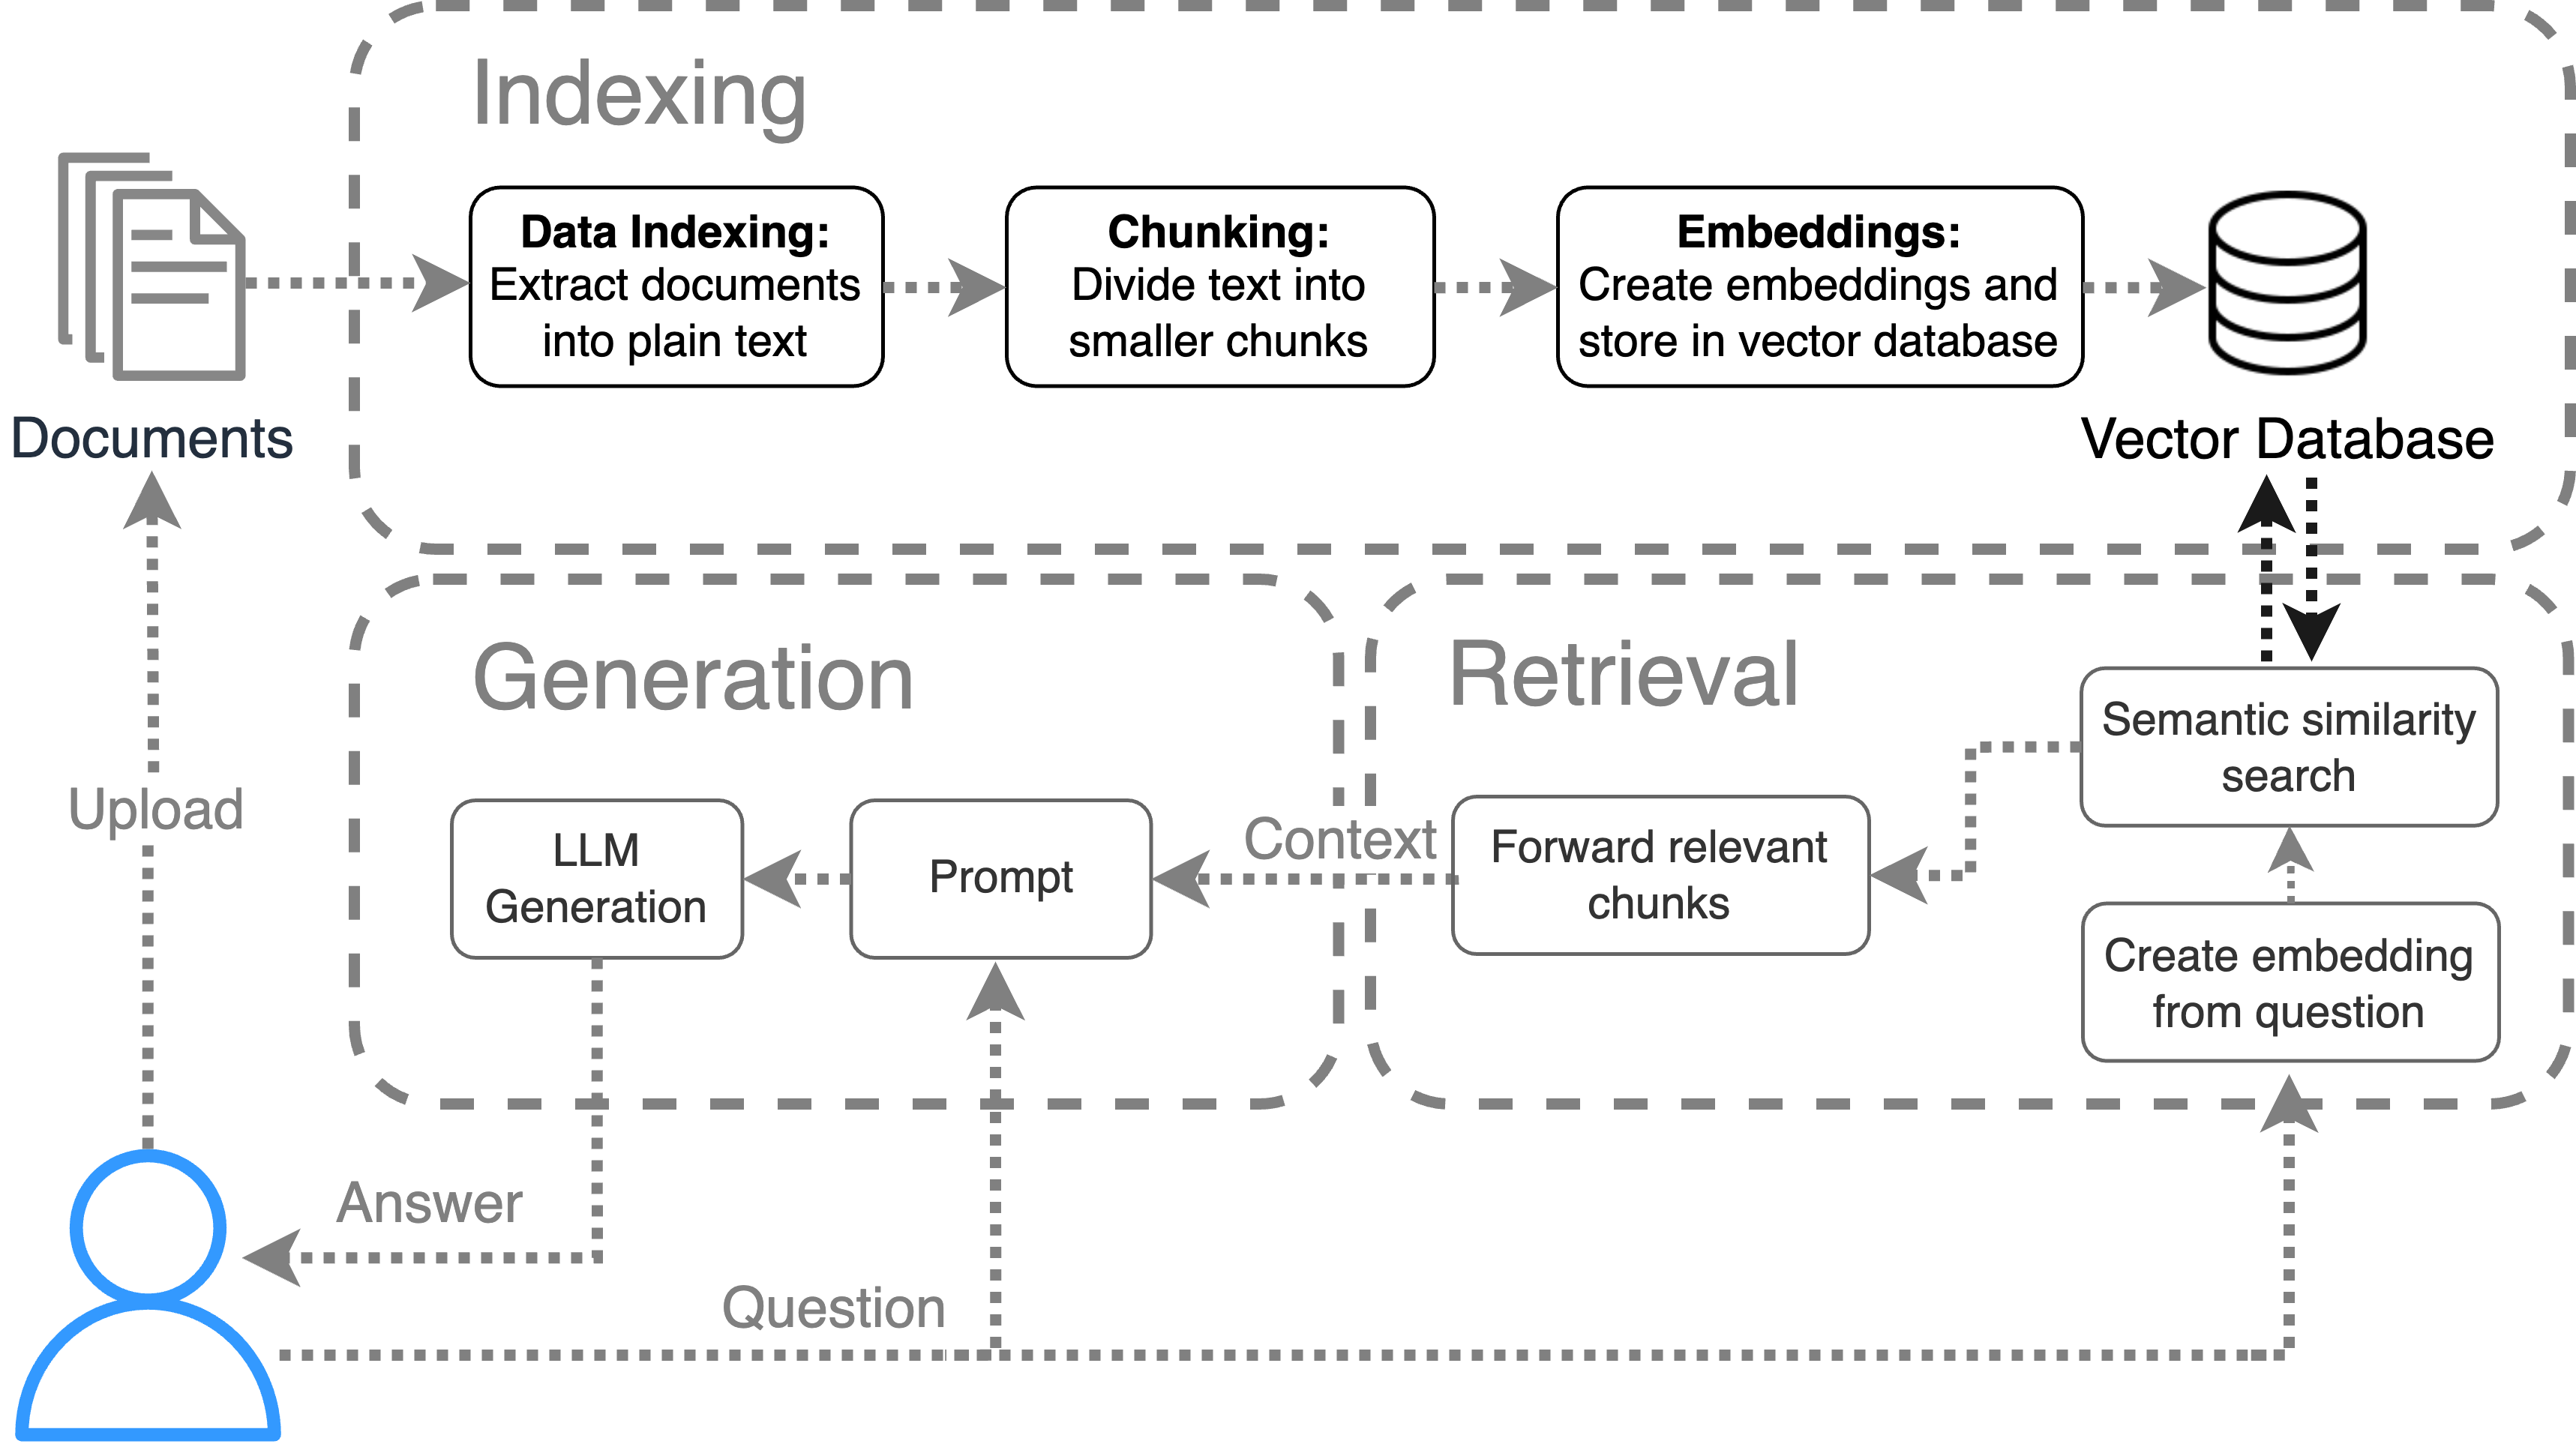
\includegraphics[width=.7\textwidth]{Figures/framework_baseline_rag.png}
    \label{fig:BaselineRAGFramework}
\end{figure}


\newpage

\subsection{GraphRAG Implementation}

Using the official Neo4j GraphRAG implementation:
\begin{itemize}
    \item HybridCypherRetriever for combining vector search with graph traversal
    \item Default parameters as specified in Neo4j documentation
    \item Entity and relationship extraction performed by LLMs during indexing
\end{itemize}

The GraphRAG system extends the baseline approach by introducing structured knowledge graph representations. During indexing, entities and their relationships are extracted from text using LLMs and stored as nodes and edges in a Neo4j database. This process is visualized in Figure~\ref{fig:GraphRAGFramework}, which outlines the main components of the GraphRAG pipeline.


\begin{figure}[h]
    \caption{GraphRAG Framework}
    \centering
    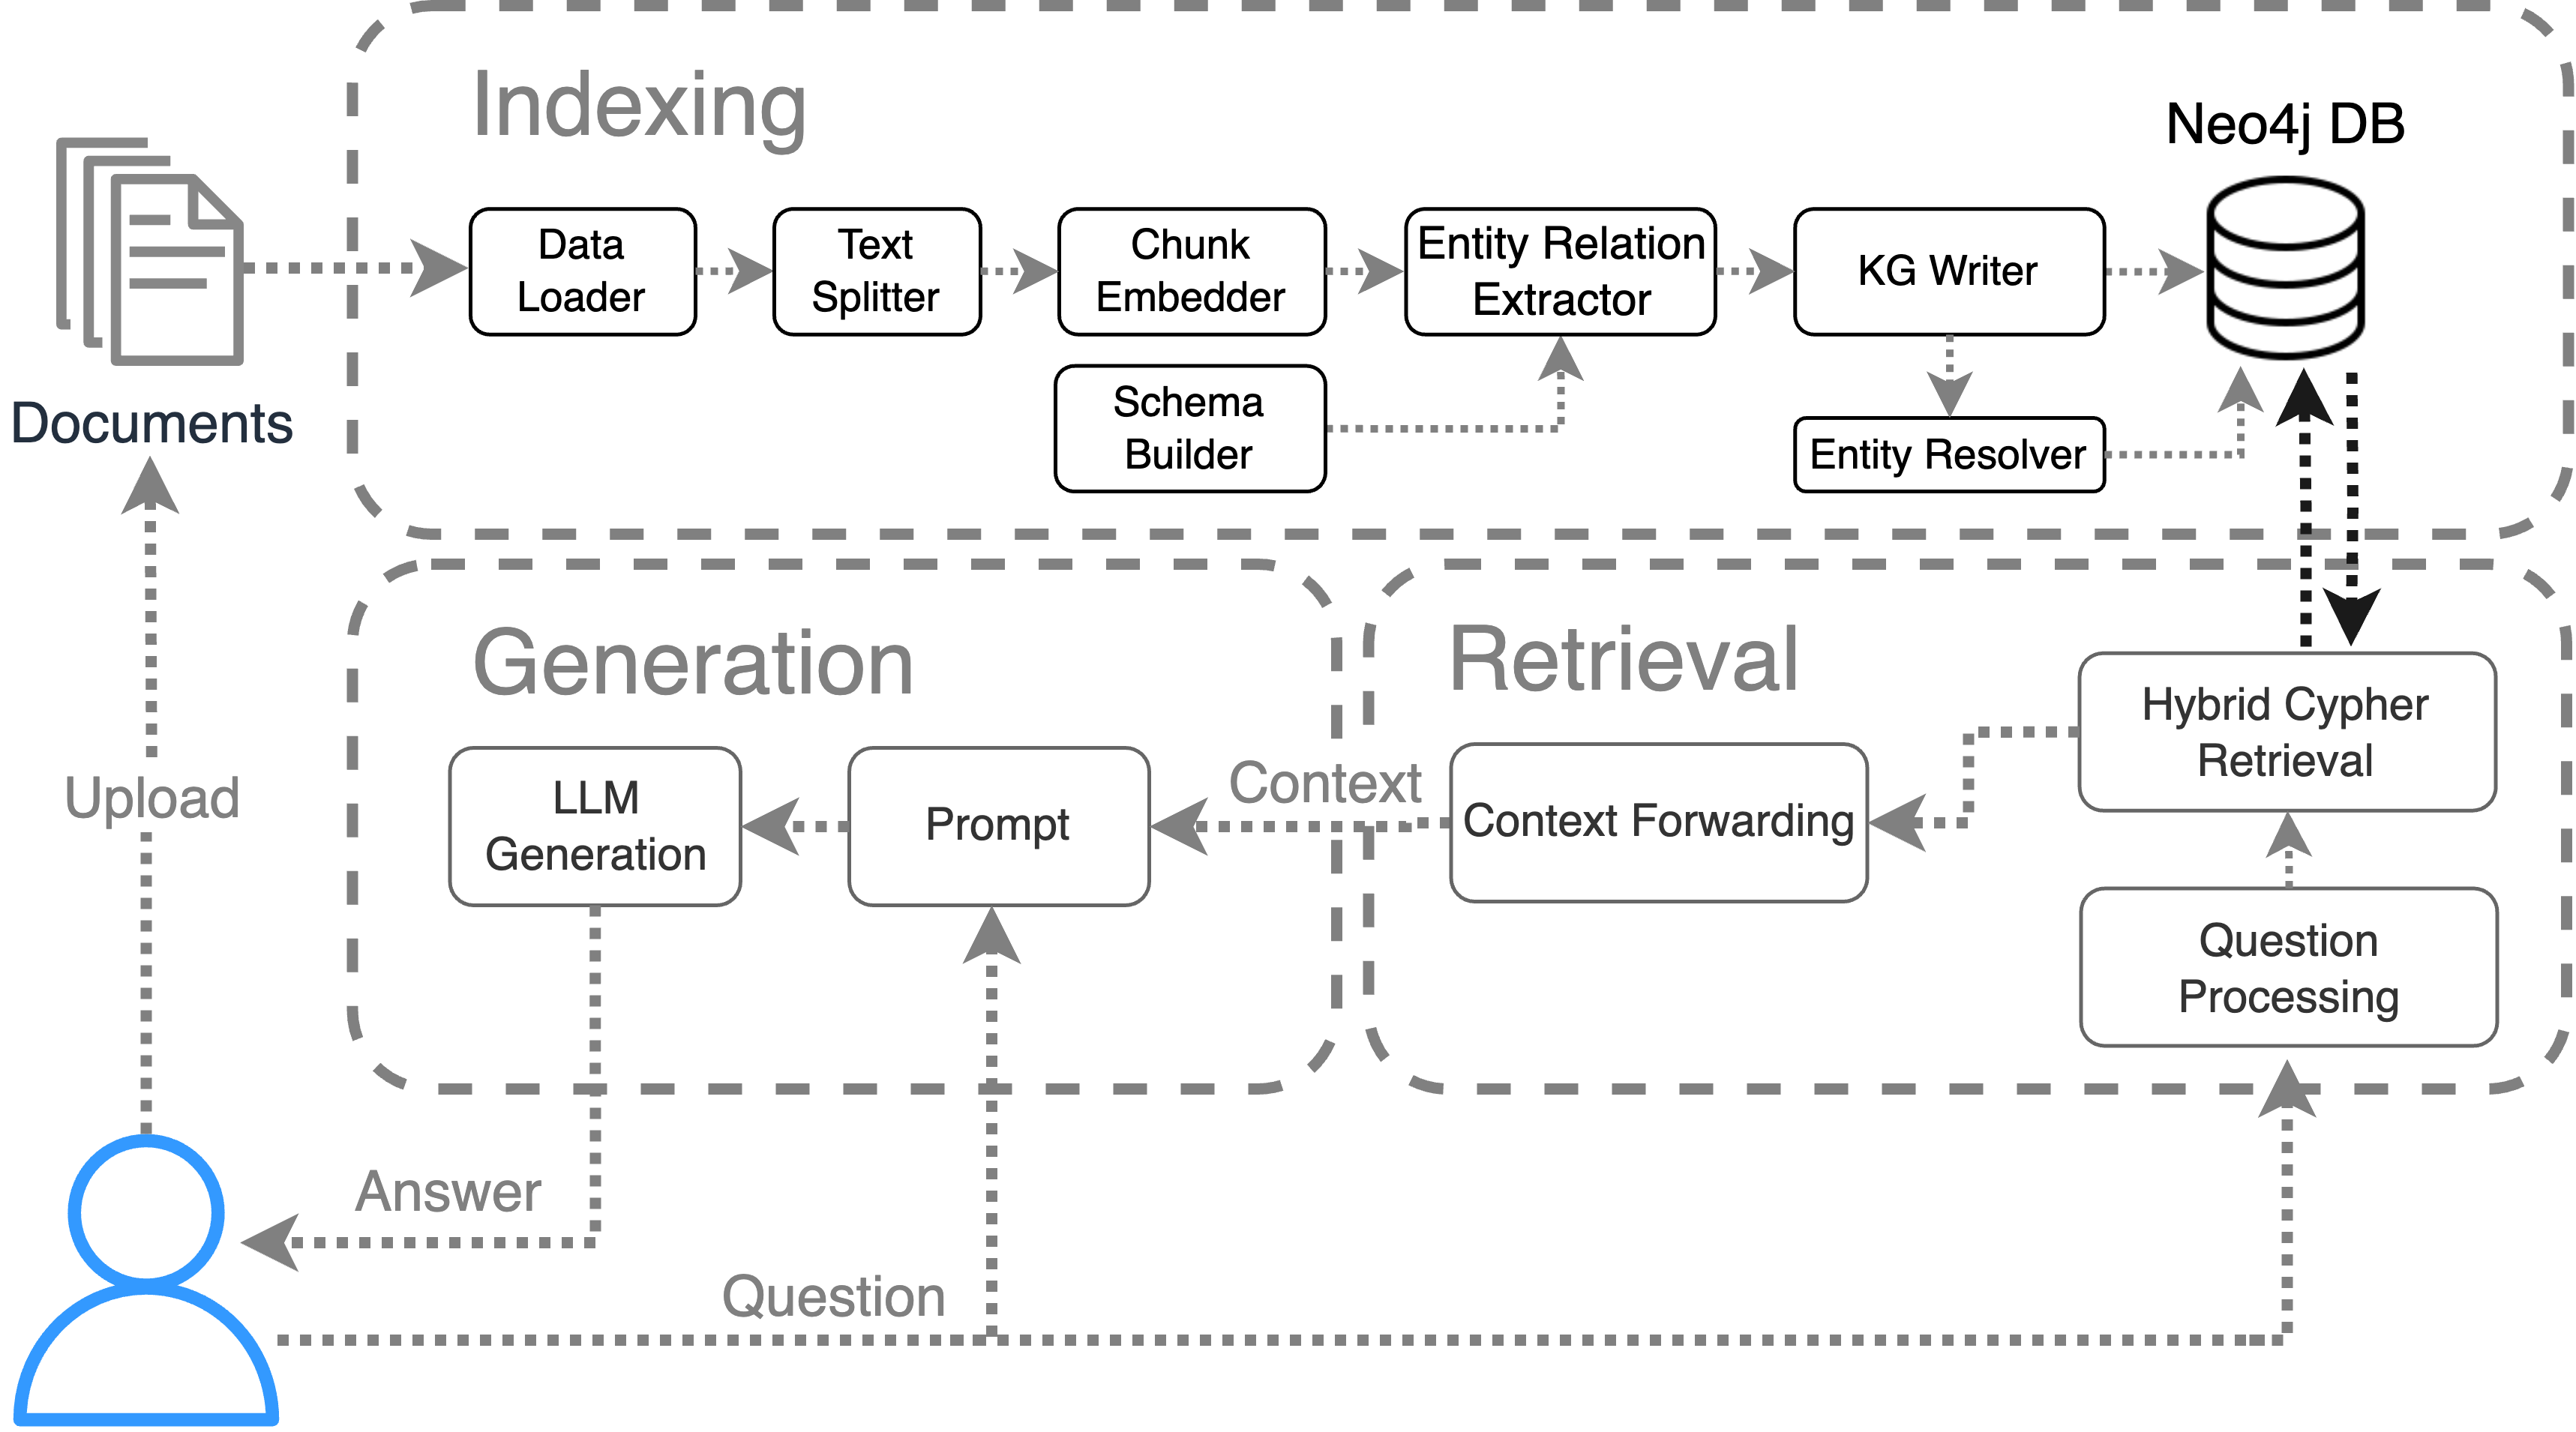
\includegraphics[width=.7\textwidth]{Figures/framework_graphrag.png}
    \label{fig:GraphRAGFramework}
\end{figure}


The retrieval process is handled by the \textit{HybridCypherRetriever}, which combines vector-based semantic retrieval with graph traversal. Retrieved nodes can be expanded through connected relationships (e.g., \texttt{:MENTIONS}, \texttt{:RELATED\_TO}) to gather additional, contextually relevant information. This hybrid process, depicted in Figure~\ref{fig:GraphRAGFrameworkRetrieval}, allows the system to integrate both implicit semantic similarity and explicit relational context.



\begin{figure}[h]
    \caption{HybridCypherRetrieval process combining semantic similarity    with graph relationships.}
    \centering
    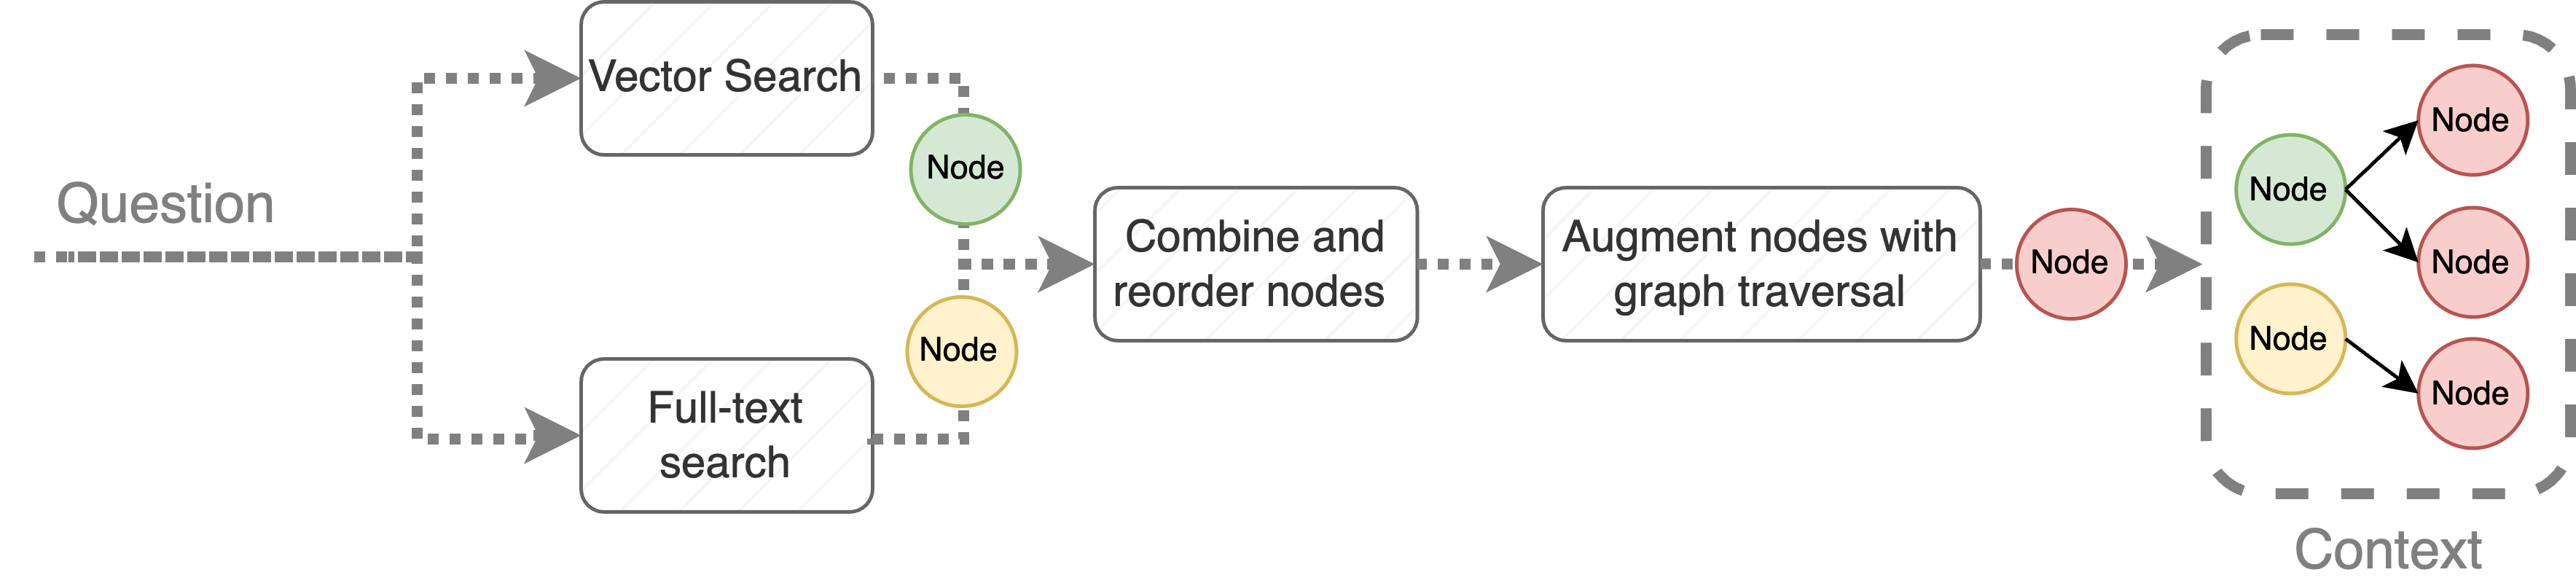
\includegraphics[width=.7\textwidth]{Figures/framework_graphrag_retrieval.png}
    \label{fig:GraphRAGFrameworkRetrieval}
\end{figure}

\subsection{Resource Tracking}

All experiments tracked:
\begin{itemize}
    \item Input and output token counts
    \item API costs (OpenAI and GroqCloud pricing)
    \item Processing time for each phase
    \item Generated graph sizes (nodes and relationships)
\end{itemize}

The implementation and dataset are publicly available at: \githuburl

























\newpage

\section{Dataset Examples}

\subsection{Sample Questions and Answers by Category}

We present representative examples from each of the six evaluation categories in VersionQA, taken directly from our dataset.

\subsubsection{Content Retrieval (Standard)}

\textbf{Q1:} What are the four categories of errors that Node.js applications generally experience?\\
\textbf{A:} The four categories are: Standard JavaScript errors, system errors, user-specified errors, and AssertionErrors.

\textbf{Q2:} What is the purpose of the error.code property in Node.js errors?\\
\textbf{A:} The error.code property is a string label that identifies the kind of error and is the most stable way to identify an error across Node.js versions.

\textbf{Q3:} What was fixed in Apache SPARK-31967?\\
\textbf{A:} SPARK-31967 fixed the issue where loading the jobs UI page took 40 seconds.

\subsubsection{Content Retrieval Complex}

\textbf{Q1:} What is the difference between assert.deepEqual() and assert.deepStrictEqual() in Node.js?\\
\textbf{A:} 'deepEqual()' allows coercion (uses '=='), while 'deepStrictEqual()' uses 'Object.is()' for strict comparison; the latter is more reliable.

\textbf{Q2:} How does assert.throws() validate errors in Node.js?\\
\textbf{A:} It checks that a function throws an error matching a specified class, RegExp, validator function, or object; throws AssertionError if validation fails.

\textbf{Q3:} What happens if no 'error' event handler is provided for an EventEmitter in Node.js?\\
\textbf{A:} The process crashes unless an 'uncaughtException' handler is registered, making proper 'error' handling essential.

\subsubsection{Content Retrieval Version-Specific}

\textbf{Q1:} What is the stability level of the assert.CallTracker in Node.js version 20.19.0?\\
\textbf{A:} Stability: 0 - Deprecated

\textbf{Q2:} What is the stability level of the assert.partialDeepStrictEqual method in Node.js version 23.11.0?\\
\textbf{A:} In Node.js v23.11.0, the stability level of the assert.partialDeepStrictEqual method is 1\_2 - Release candidate.

\textbf{Q3:} What type of release is Apache Spark 2.4.7?\\
\textbf{A:} Spark 2.4.7 is a maintenance release containing stability, correctness, and security fixes.

\subsubsection{Version Listing \& Inquiry}

\textbf{Q1:} What is the latest NodeJs version you know of?\\
\textbf{A:} 23.11.0

\textbf{Q2:} What Apache Spark versions are available?\\
\textbf{A:} Version 2.4.7, Version 3.3.4, Version 3.4.4, Version 3.5.3, Version 3.5.4, Version 3.5.5.

\textbf{Q3:} Does NodeJs version 21.7.3 exist in the system?\\
\textbf{A:} Yes

\textbf{Q4:} How many Bootstrap versions are you aware of?\\
\textbf{A:} 5.2.3, 5.3.1, 5.3.2, 5.3.3, 5.3.4, 5.3.5. That makes a total of six versions.

\subsubsection{Change Retrieval (Explicit)}

\textbf{Q1:} What dependency was upgraded in Apache Spark 3.5.5?\\
\textbf{A:} Avro was upgraded to version 1.11.4 in Spark 3.5.5.

\textbf{Q2:} What change was made to the way badges handle text readability in Bootstrap v5.3.3?\\
\textbf{A:} Badges now use the .text-bg-* text utilities to ensure that the text is always readable, especially when customized colors differ in light and dark modes.

\textbf{Q3:} What was fixed in the selector engine in Bootstrap v5.3.3?\\
\textbf{A:} A regression in the selector engine that wasn't able to handle multiple IDs anymore was fixed.

\subsubsection{Change Retrieval (Implicit)}

\textbf{Q1:} When was the assert method partialDeepStrictEqual added to Node.js Assert?\\
\textbf{A:} The assert.partialDeepStrictEqual method was added to Node.js in version 22.14.0.

\textbf{Q2:} With what Node.js version was error code ERR\_ACCESS\_DENIED added?\\
\textbf{A:} The error code ERR\_ACCESS\_DENIED was added in Node.js version 16.20.2.

\textbf{Q3:} Was the CallTracker object introduced as new feature in Node.js Assert version 14.21.3?\\
\textbf{A:} Yes, the CallTracker object was introduced as a new feature in Node.js Assert version 14.21.3.

\subsection{Dataset Statistics}

Based on the dataset composition described in Section~\ref{sec:dataset}.

\begin{table}[hb]
\centering
\small
\caption{Dataset distribution showing 60\% of queries require version-aware reasoning.}
\begin{tabular}{lcc}
\hline
\textbf{Category} & \textbf{Q\&A Pairs} & \textbf{Version-Sensitive} \\ \hline
Content Retrieval & 20 & No \\
Content Retrieval Complex & 20 & No \\
Content Retrieval Version-Specific & 20 & Yes \\
Version Listing \& Inquiry & 20 & Yes \\
Change Retrieval (Explicit) & 10 & Yes \\
Change Retrieval (Implicit) & 10 & Yes \\ \hline
\textbf{Total} & \textbf{100} & \textbf{60\%} \\ \hline
\end{tabular}
\label{tab:dataset_statistics}
\end{table}

